%%%%%%%%%%%%%%%%%%%%%%%%%%%%%%%%%%%%%%%%%%%%%%%%%%%%%%%
%          Penetration Test Report Template           %
%                     cyber@cfreg                     %
%             https://hack.newhaven.edu/              %
%                                                     %
%                    Contributors:                    %
% TJ Balon - https://github.com/tjbalon               %
% Samuel Zurowski - https://github.com/samuelzurowski %
% Charles Barone - https://github.com/CharlesBarone   %
%%%%%%%%%%%%%%%%%%%%%%%%%%%%%%%%%%%%%%%%%%%%%%%%%%%%%%%
\printbibliography
\newpage
\newpage
\appendix
\appendixpage
\addappheadtotoc

% This should be a network topology that represents the in scope network from the engagement
% The example below was made using Lucidchart (https://lucid.app):
\section{Network Topology}
    \label{appendix:A}
    \begin{figure}[H]
        \centering
        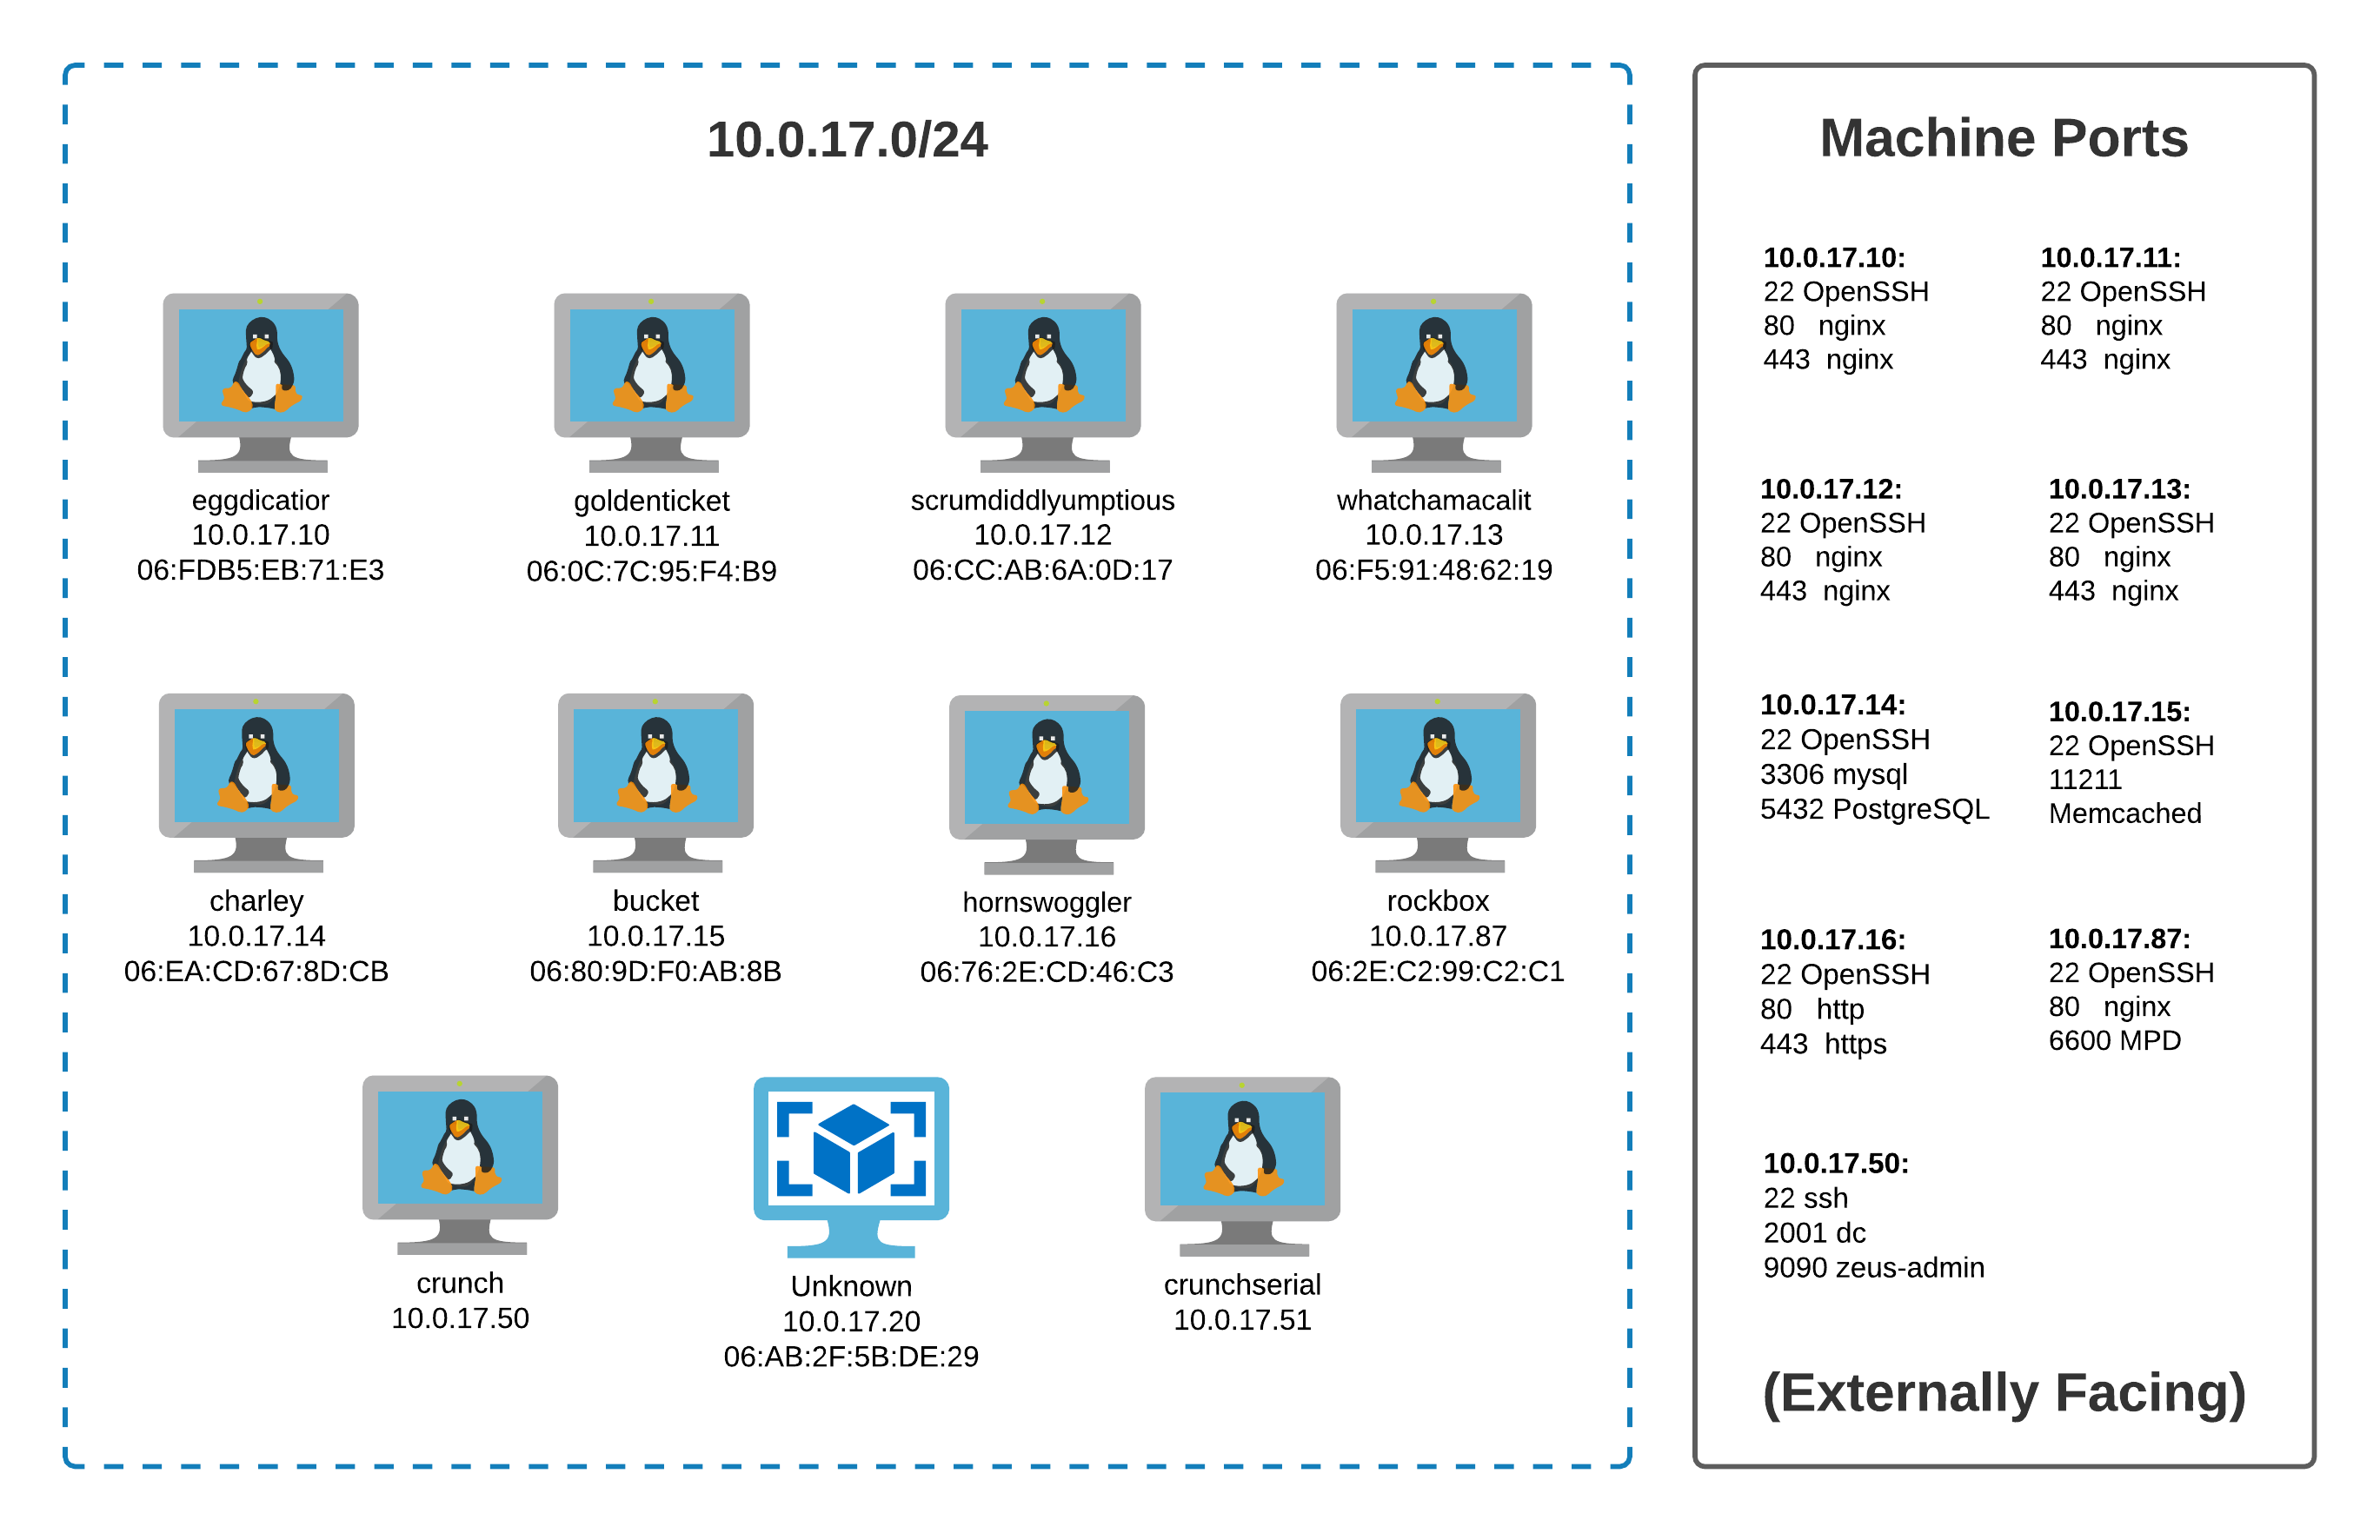
\includegraphics[width=\textwidth]{images/general/topology.PNG}
        \caption{Network Topology}
        \label{fig:nettopology}
    \end{figure}

% This should be a table of all tools utilized during the engagement.
% An example of what this may look like is included below:
\newpage
\section{Tools}
    \begin{table}[H]
    \renewcommand{\arraystretch}{1.25}
        \centering
        \begin{tabular}{|l|p{12em}|p{18em}|}\hline
            \textbf{Name} & \textbf{Description} & \textbf{Link} \\\hline
            Nmap & Network and vulnerability scanner & \url{https://nmap.org/} \\\hline
            Metasploit & Exploitation framework & \url{https://github.com/rapid7/metasploit-framework} \\\hline
            DIRB & Directory Brute Force Tool & \url{https://github.com/v0re/dirb} \\\hline
            Gobuster & Directory Brute Force Tool & \url{https://github.com/OJ/gobuster} \\\hline
            Meterpreter & Reverse Shell & \url{https://github.com/rapid7/meterpreter} \\\hline
            Crowbar & Brute forcing tool & \url{https://github.com/galkan/crowbar} \\\hline
            netcat & Network utility & \url{https://github.com/diegocr/netcat}\\\hline
            hydra & Brute Forcing tool & \url{https://github.com/vanhauser-thc/thc-hydra}\\\hline
            Wireshark & Network traffic analyzer & \url{https://www.wireshark.org/}\\\hline
            Portswigger Burp Suite & Web traffic analysis tool & \url{https://portswigger.net/burp} \\\hline
            psql & PostgreSQL interactive terminal & \url{https://www.postgresql.org/docs/13/app-psql.html} \\ \hline
        \end{tabular}
    \end{table}